% Created by tikzDevice version 0.8.1 on 2015-11-17 12:26:03
% !TEX encoding = UTF-8 Unicode
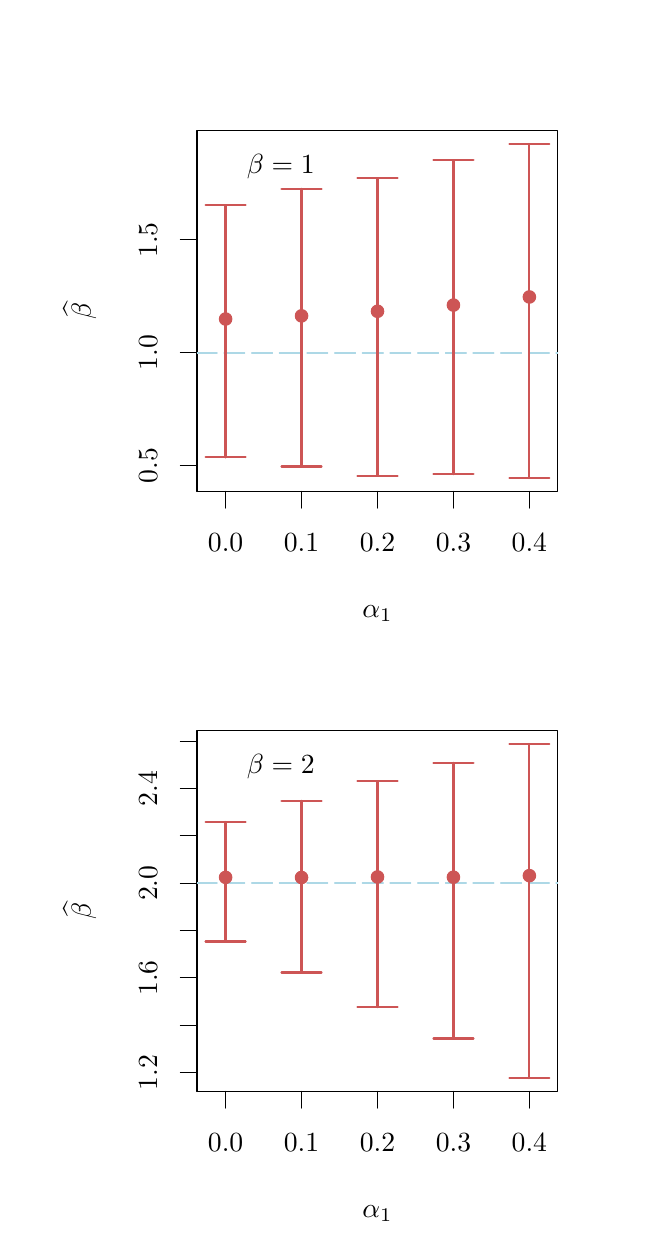
\begin{tikzpicture}[x=1pt,y=1pt]
\definecolor{fillColor}{RGB}{255,255,255}
\path[use as bounding box,fill=fillColor,fill opacity=0.00] (0,0) rectangle (216.81,433.62);
\begin{scope}
\path[clip] ( 61.20,266.01) rectangle (191.61,396.42);
\definecolor{drawColor}{RGB}{255,255,255}
\definecolor{fillColor}{RGB}{255,255,255}

\path[draw=drawColor,line width= 0.4pt,line join=round,line cap=round,fill=fillColor] ( 71.52,328.34) circle (  2.25);

\path[draw=drawColor,line width= 0.4pt,line join=round,line cap=round,fill=fillColor] ( 98.96,329.48) circle (  2.25);

\path[draw=drawColor,line width= 0.4pt,line join=round,line cap=round,fill=fillColor] (126.41,331.14) circle (  2.25);

\path[draw=drawColor,line width= 0.4pt,line join=round,line cap=round,fill=fillColor] (153.85,333.37) circle (  2.25);

\path[draw=drawColor,line width= 0.4pt,line join=round,line cap=round,fill=fillColor] (181.29,336.31) circle (  2.25);
\end{scope}
\begin{scope}
\path[clip] (  0.00,  0.00) rectangle (216.81,433.62);
\definecolor{drawColor}{RGB}{0,0,0}

\path[draw=drawColor,line width= 0.4pt,line join=round,line cap=round] ( 71.52,266.01) -- (181.29,266.01);

\path[draw=drawColor,line width= 0.4pt,line join=round,line cap=round] ( 71.52,266.01) -- ( 71.52,260.01);

\path[draw=drawColor,line width= 0.4pt,line join=round,line cap=round] ( 98.96,266.01) -- ( 98.96,260.01);

\path[draw=drawColor,line width= 0.4pt,line join=round,line cap=round] (126.41,266.01) -- (126.41,260.01);

\path[draw=drawColor,line width= 0.4pt,line join=round,line cap=round] (153.85,266.01) -- (153.85,260.01);

\path[draw=drawColor,line width= 0.4pt,line join=round,line cap=round] (181.29,266.01) -- (181.29,260.01);

\node[text=drawColor,anchor=base,inner sep=0pt, outer sep=0pt, scale=  1.00] at ( 71.52,244.41) {0.0};

\node[text=drawColor,anchor=base,inner sep=0pt, outer sep=0pt, scale=  1.00] at ( 98.96,244.41) {0.1};

\node[text=drawColor,anchor=base,inner sep=0pt, outer sep=0pt, scale=  1.00] at (126.41,244.41) {0.2};

\node[text=drawColor,anchor=base,inner sep=0pt, outer sep=0pt, scale=  1.00] at (153.85,244.41) {0.3};

\node[text=drawColor,anchor=base,inner sep=0pt, outer sep=0pt, scale=  1.00] at (181.29,244.41) {0.4};

\path[draw=drawColor,line width= 0.4pt,line join=round,line cap=round] ( 61.20,275.35) -- ( 61.20,356.94);

\path[draw=drawColor,line width= 0.4pt,line join=round,line cap=round] ( 61.20,275.35) -- ( 55.20,275.35);

\path[draw=drawColor,line width= 0.4pt,line join=round,line cap=round] ( 61.20,316.14) -- ( 55.20,316.14);

\path[draw=drawColor,line width= 0.4pt,line join=round,line cap=round] ( 61.20,356.94) -- ( 55.20,356.94);

\node[text=drawColor,rotate= 90.00,anchor=base,inner sep=0pt, outer sep=0pt, scale=  1.00] at ( 46.80,275.35) {0.5};

\node[text=drawColor,rotate= 90.00,anchor=base,inner sep=0pt, outer sep=0pt, scale=  1.00] at ( 46.80,316.14) {1.0};

\node[text=drawColor,rotate= 90.00,anchor=base,inner sep=0pt, outer sep=0pt, scale=  1.00] at ( 46.80,356.94) {1.5};

\path[draw=drawColor,line width= 0.4pt,line join=round,line cap=round] ( 61.20,266.01) --
	(191.61,266.01) --
	(191.61,396.42) --
	( 61.20,396.42) --
	( 61.20,266.01);
\end{scope}
\begin{scope}
\path[clip] (  0.00,216.81) rectangle (216.81,433.62);
\definecolor{drawColor}{RGB}{0,0,0}

\node[text=drawColor,anchor=base,inner sep=0pt, outer sep=0pt, scale=  1.00] at (126.41,220.41) {$\alpha_1$};

\node[text=drawColor,rotate= 90.00,anchor=base,inner sep=0pt, outer sep=0pt, scale=  1.00] at ( 22.80,331.22) {$\widehat{\beta}$};
\end{scope}
\begin{scope}
\path[clip] ( 61.20,266.01) rectangle (191.61,396.42);
\definecolor{drawColor}{RGB}{0,0,0}

\node[text=drawColor,anchor=base west,inner sep=0pt, outer sep=0pt, scale=  1.00] at ( 79.20,380.98) {$\beta=1$};
\definecolor{drawColor}{RGB}{173,216,230}

\path[draw=drawColor,line width= 0.8pt,dash pattern=on 7pt off 3pt ,line join=round,line cap=round] ( 61.20,316.14) -- (191.61,316.14);

\path[draw=drawColor,line width= 0.8pt,dash pattern=on 7pt off 3pt ,line join=round,line cap=round] ( 61.20,316.14) -- (191.61,316.14);

\path[draw=drawColor,line width= 0.8pt,dash pattern=on 7pt off 3pt ,line join=round,line cap=round] ( 61.20,316.14) -- (191.61,316.14);

\path[draw=drawColor,line width= 0.8pt,dash pattern=on 7pt off 3pt ,line join=round,line cap=round] ( 61.20,316.14) -- (191.61,316.14);

\path[draw=drawColor,line width= 0.8pt,dash pattern=on 7pt off 3pt ,line join=round,line cap=round] ( 61.20,316.14) -- (191.61,316.14);
\definecolor{drawColor}{RGB}{205,85,85}

\path[draw=drawColor,line width= 0.8pt,line join=round,line cap=round] ( 71.52,278.34) -- ( 71.52,369.48);

\path[draw=drawColor,line width= 0.8pt,line join=round,line cap=round] ( 64.29,278.34) --
	( 71.52,278.34) --
	( 78.75,278.34);

\path[draw=drawColor,line width= 0.8pt,line join=round,line cap=round] ( 78.75,369.48) --
	( 71.52,369.48) --
	( 64.29,369.48);

\path[draw=drawColor,line width= 0.8pt,line join=round,line cap=round] ( 98.96,275.02) -- ( 98.96,375.35);

\path[draw=drawColor,line width= 0.8pt,line join=round,line cap=round] ( 91.73,275.02) --
	( 98.96,275.02) --
	(106.19,275.02);

\path[draw=drawColor,line width= 0.8pt,line join=round,line cap=round] (106.19,375.35) --
	( 98.96,375.35) --
	( 91.73,375.35);

\path[draw=drawColor,line width= 0.8pt,line join=round,line cap=round] (126.41,271.75) -- (126.41,379.21);

\path[draw=drawColor,line width= 0.8pt,line join=round,line cap=round] (119.18,271.75) --
	(126.41,271.75) --
	(133.63,271.75);

\path[draw=drawColor,line width= 0.8pt,line join=round,line cap=round] (133.63,379.21) --
	(126.41,379.21) --
	(119.18,379.21);

\path[draw=drawColor,line width= 0.8pt,line join=round,line cap=round] (153.85,272.29) -- (153.85,385.66);

\path[draw=drawColor,line width= 0.8pt,line join=round,line cap=round] (146.62,272.29) --
	(153.85,272.29) --
	(161.08,272.29);

\path[draw=drawColor,line width= 0.8pt,line join=round,line cap=round] (161.08,385.66) --
	(153.85,385.66) --
	(146.62,385.66);

\path[draw=drawColor,line width= 0.8pt,line join=round,line cap=round] (181.29,270.84) -- (181.29,391.59);

\path[draw=drawColor,line width= 0.8pt,line join=round,line cap=round] (174.06,270.84) --
	(181.29,270.84) --
	(188.52,270.84);

\path[draw=drawColor,line width= 0.8pt,line join=round,line cap=round] (188.52,391.59) --
	(181.29,391.59) --
	(174.06,391.59);
\definecolor{fillColor}{RGB}{205,85,85}

\path[draw=drawColor,line width= 0.4pt,line join=round,line cap=round,fill=fillColor] ( 71.52,328.34) circle (  2.25);

\path[draw=drawColor,line width= 0.4pt,line join=round,line cap=round,fill=fillColor] ( 98.96,329.48) circle (  2.25);

\path[draw=drawColor,line width= 0.4pt,line join=round,line cap=round,fill=fillColor] (126.41,331.14) circle (  2.25);

\path[draw=drawColor,line width= 0.4pt,line join=round,line cap=round,fill=fillColor] (153.85,333.37) circle (  2.25);

\path[draw=drawColor,line width= 0.4pt,line join=round,line cap=round,fill=fillColor] (181.29,336.31) circle (  2.25);
\end{scope}
\begin{scope}
\path[clip] ( 61.20, 49.20) rectangle (191.61,179.61);
\definecolor{drawColor}{RGB}{255,255,255}
\definecolor{fillColor}{RGB}{255,255,255}

\path[draw=drawColor,line width= 0.4pt,line join=round,line cap=round,fill=fillColor] ( 71.52,126.58) circle (  2.25);

\path[draw=drawColor,line width= 0.4pt,line join=round,line cap=round,fill=fillColor] ( 98.96,126.54) circle (  2.25);

\path[draw=drawColor,line width= 0.4pt,line join=round,line cap=round,fill=fillColor] (126.41,126.72) circle (  2.25);

\path[draw=drawColor,line width= 0.4pt,line join=round,line cap=round,fill=fillColor] (153.85,126.64) circle (  2.25);

\path[draw=drawColor,line width= 0.4pt,line join=round,line cap=round,fill=fillColor] (181.29,127.20) circle (  2.25);
\end{scope}
\begin{scope}
\path[clip] (  0.00,  0.00) rectangle (216.81,433.62);
\definecolor{drawColor}{RGB}{0,0,0}

\path[draw=drawColor,line width= 0.4pt,line join=round,line cap=round] ( 71.52, 49.20) -- (181.29, 49.20);

\path[draw=drawColor,line width= 0.4pt,line join=round,line cap=round] ( 71.52, 49.20) -- ( 71.52, 43.20);

\path[draw=drawColor,line width= 0.4pt,line join=round,line cap=round] ( 98.96, 49.20) -- ( 98.96, 43.20);

\path[draw=drawColor,line width= 0.4pt,line join=round,line cap=round] (126.41, 49.20) -- (126.41, 43.20);

\path[draw=drawColor,line width= 0.4pt,line join=round,line cap=round] (153.85, 49.20) -- (153.85, 43.20);

\path[draw=drawColor,line width= 0.4pt,line join=round,line cap=round] (181.29, 49.20) -- (181.29, 43.20);

\node[text=drawColor,anchor=base,inner sep=0pt, outer sep=0pt, scale=  1.00] at ( 71.52, 27.60) {0.0};

\node[text=drawColor,anchor=base,inner sep=0pt, outer sep=0pt, scale=  1.00] at ( 98.96, 27.60) {0.1};

\node[text=drawColor,anchor=base,inner sep=0pt, outer sep=0pt, scale=  1.00] at (126.41, 27.60) {0.2};

\node[text=drawColor,anchor=base,inner sep=0pt, outer sep=0pt, scale=  1.00] at (153.85, 27.60) {0.3};

\node[text=drawColor,anchor=base,inner sep=0pt, outer sep=0pt, scale=  1.00] at (181.29, 27.60) {0.4};

\path[draw=drawColor,line width= 0.4pt,line join=round,line cap=round] ( 61.20, 56.06) -- ( 61.20,175.78);

\path[draw=drawColor,line width= 0.4pt,line join=round,line cap=round] ( 61.20, 56.06) -- ( 55.20, 56.06);

\path[draw=drawColor,line width= 0.4pt,line join=round,line cap=round] ( 61.20, 73.16) -- ( 55.20, 73.16);

\path[draw=drawColor,line width= 0.4pt,line join=round,line cap=round] ( 61.20, 90.26) -- ( 55.20, 90.26);

\path[draw=drawColor,line width= 0.4pt,line join=round,line cap=round] ( 61.20,107.37) -- ( 55.20,107.37);

\path[draw=drawColor,line width= 0.4pt,line join=round,line cap=round] ( 61.20,124.47) -- ( 55.20,124.47);

\path[draw=drawColor,line width= 0.4pt,line join=round,line cap=round] ( 61.20,141.58) -- ( 55.20,141.58);

\path[draw=drawColor,line width= 0.4pt,line join=round,line cap=round] ( 61.20,158.68) -- ( 55.20,158.68);

\path[draw=drawColor,line width= 0.4pt,line join=round,line cap=round] ( 61.20,175.78) -- ( 55.20,175.78);

\node[text=drawColor,rotate= 90.00,anchor=base,inner sep=0pt, outer sep=0pt, scale=  1.00] at ( 46.80, 56.06) {1.2};

\node[text=drawColor,rotate= 90.00,anchor=base,inner sep=0pt, outer sep=0pt, scale=  1.00] at ( 46.80, 90.26) {1.6};

\node[text=drawColor,rotate= 90.00,anchor=base,inner sep=0pt, outer sep=0pt, scale=  1.00] at ( 46.80,124.47) {2.0};

\node[text=drawColor,rotate= 90.00,anchor=base,inner sep=0pt, outer sep=0pt, scale=  1.00] at ( 46.80,158.68) {2.4};

\path[draw=drawColor,line width= 0.4pt,line join=round,line cap=round] ( 61.20, 49.20) --
	(191.61, 49.20) --
	(191.61,179.61) --
	( 61.20,179.61) --
	( 61.20, 49.20);
\end{scope}
\begin{scope}
\path[clip] (  0.00,  0.00) rectangle (216.81,216.81);
\definecolor{drawColor}{RGB}{0,0,0}

\node[text=drawColor,anchor=base,inner sep=0pt, outer sep=0pt, scale=  1.00] at (126.41,  3.60) {$\alpha_1$};

\node[text=drawColor,rotate= 90.00,anchor=base,inner sep=0pt, outer sep=0pt, scale=  1.00] at ( 22.80,114.41) {$\widehat{\beta}$};
\end{scope}
\begin{scope}
\path[clip] ( 61.20, 49.20) rectangle (191.61,179.61);
\definecolor{drawColor}{RGB}{0,0,0}

\node[text=drawColor,anchor=base west,inner sep=0pt, outer sep=0pt, scale=  1.00] at ( 79.20,164.17) {$\beta=2$};
\definecolor{drawColor}{RGB}{173,216,230}

\path[draw=drawColor,line width= 0.8pt,dash pattern=on 7pt off 3pt ,line join=round,line cap=round] ( 61.20,124.47) -- (191.61,124.47);

\path[draw=drawColor,line width= 0.8pt,dash pattern=on 7pt off 3pt ,line join=round,line cap=round] ( 61.20,124.47) -- (191.61,124.47);

\path[draw=drawColor,line width= 0.8pt,dash pattern=on 7pt off 3pt ,line join=round,line cap=round] ( 61.20,124.47) -- (191.61,124.47);

\path[draw=drawColor,line width= 0.8pt,dash pattern=on 7pt off 3pt ,line join=round,line cap=round] ( 61.20,124.47) -- (191.61,124.47);

\path[draw=drawColor,line width= 0.8pt,dash pattern=on 7pt off 3pt ,line join=round,line cap=round] ( 61.20,124.47) -- (191.61,124.47);
\definecolor{drawColor}{RGB}{205,85,85}

\path[draw=drawColor,line width= 0.8pt,line join=round,line cap=round] ( 71.52,103.38) -- ( 71.52,146.61);

\path[draw=drawColor,line width= 0.8pt,line join=round,line cap=round] ( 64.29,103.38) --
	( 71.52,103.38) --
	( 78.75,103.38);

\path[draw=drawColor,line width= 0.8pt,line join=round,line cap=round] ( 78.75,146.61) --
	( 71.52,146.61) --
	( 64.29,146.61);

\path[draw=drawColor,line width= 0.8pt,line join=round,line cap=round] ( 98.96, 92.24) -- ( 98.96,154.22);

\path[draw=drawColor,line width= 0.8pt,line join=round,line cap=round] ( 91.73, 92.24) --
	( 98.96, 92.24) --
	(106.19, 92.24);

\path[draw=drawColor,line width= 0.8pt,line join=round,line cap=round] (106.19,154.22) --
	( 98.96,154.22) --
	( 91.73,154.22);

\path[draw=drawColor,line width= 0.8pt,line join=round,line cap=round] (126.41, 79.70) -- (126.41,161.30);

\path[draw=drawColor,line width= 0.8pt,line join=round,line cap=round] (119.18, 79.70) --
	(126.41, 79.70) --
	(133.63, 79.70);

\path[draw=drawColor,line width= 0.8pt,line join=round,line cap=round] (133.63,161.30) --
	(126.41,161.30) --
	(119.18,161.30);

\path[draw=drawColor,line width= 0.8pt,line join=round,line cap=round] (153.85, 68.32) -- (153.85,167.95);

\path[draw=drawColor,line width= 0.8pt,line join=round,line cap=round] (146.62, 68.32) --
	(153.85, 68.32) --
	(161.08, 68.32);

\path[draw=drawColor,line width= 0.8pt,line join=round,line cap=round] (161.08,167.95) --
	(153.85,167.95) --
	(146.62,167.95);

\path[draw=drawColor,line width= 0.8pt,line join=round,line cap=round] (181.29, 54.03) -- (181.29,174.78);

\path[draw=drawColor,line width= 0.8pt,line join=round,line cap=round] (174.06, 54.03) --
	(181.29, 54.03) --
	(188.52, 54.03);

\path[draw=drawColor,line width= 0.8pt,line join=round,line cap=round] (188.52,174.78) --
	(181.29,174.78) --
	(174.06,174.78);
\definecolor{fillColor}{RGB}{205,85,85}

\path[draw=drawColor,line width= 0.4pt,line join=round,line cap=round,fill=fillColor] ( 71.52,126.58) circle (  2.25);

\path[draw=drawColor,line width= 0.4pt,line join=round,line cap=round,fill=fillColor] ( 98.96,126.54) circle (  2.25);

\path[draw=drawColor,line width= 0.4pt,line join=round,line cap=round,fill=fillColor] (126.41,126.72) circle (  2.25);

\path[draw=drawColor,line width= 0.4pt,line join=round,line cap=round,fill=fillColor] (153.85,126.64) circle (  2.25);

\path[draw=drawColor,line width= 0.4pt,line join=round,line cap=round,fill=fillColor] (181.29,127.20) circle (  2.25);
\end{scope}
\end{tikzpicture}
